\subsection{Robinson Projektion}
\label{sec:robinson}
Die Robinson Projektion ist eine globale Projektion. Die Erde wird hier annähernd Oval dargestellt. Die Pole werden allerdings in dieser Darstellung nicht abgedeckt. Breitenkreise werden in der Robinson Projektion als Geraden dargestellt. Bei dieser Darstellung wurden die Verzerrungen reduziert. Nachteil der Robinson Projektion ist das die Pole nicht erfasst werden.\\

\begin{figure}[hbtp]
\centering
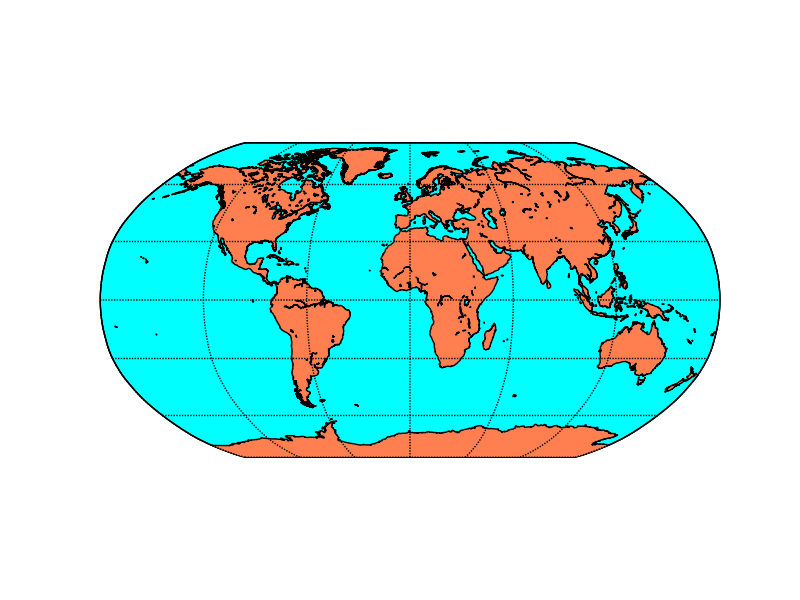
\includegraphics[scale=0.5,origin=c]{/Users/student/seminar/Kartendarstellungen/seminar/robin} \caption{Robinson Projektion}
\end{figure}
\newpage 